\renewcommand{\theequation}{\theenumi}
\begin{enumerate}[label=\arabic*.,ref=\thesection.\theenumi]
\numberwithin{equation}{enumi}

\item An apache helicopter of the enemy is flying along the curve given by 
	\label{prob:dist_pt_parab}
\begin{align}
\label{eq:dist_pt_parab}
y = x^2 +7
\end{align}
%
A soldier, placed at 
\begin{align}
\vec{P} = \myvec{3\\7}.  
\end{align}
%
wants to shoot the heicopter when it is nearest to him.  Express this as an optimization problem.
%\item
%Express the problem of 
%finding the point on the curve 
%\begin{align}
%\label{eq:dist_pt_parab}
%x^2 = 2y
%\end{align}
%%
%nearest to the point 
%\begin{align}
%\vec{P} = \myvec{0\\5}.  
%\end{align}
%%
%as an optiimization problem.
\\
\solution The given problem can be expressed as
\begin{align}
\label{eq:qp_dist_pt_parab}
\min_{\vec{x}}\norm{\vec{x}-\vec{P}}^2
\\
\text{s.t. }\vec{x}^T\vec{V}\vec{x} + \vec{u}^T\vec{x}  +d = 0
\end{align}
%
where
%
\begin{align}
\vec{V} &= \myvec{1 & 0\\0 & 0}
\\
\vec{u} &= -\myvec{0 \\ 1}
\\
d &= 7
\end{align}
\item Show that the constraint in \ref{eq:qp_dist_pt_parab} is nonconvex.
\item Show that the following {\em relaxation} makes \eqref{eq:qp_dist_pt_parab} a convex optimization problem.
%
\begin{align}
\label{eq:qp_dist_pt_parab_conv}
\min_{\vec{x}}\brak{\vec{x}-\vec{P}}^T\brak{\vec{x}-\vec{P}}
\\
\text{s.t. }\vec{x}^T\vec{V}\vec{x} + \vec{u}^T\vec{x}  \le 0
\end{align}
%
%
\item Solve \eqref{eq:qp_dist_pt_parab_conv} using cvxpy.
\\
\solution  The following code yields the minimum distance as 2.236 and the nearest point on the curve as
%
\begin{align}
\vec{Q} &= \myvec{1\\8}
\end{align}

\begin{lstlisting}
codes/qp_cvx.py
\end{lstlisting}

\item Solve \eqref{eq:qp_dist_pt_parab_conv} using the method of Lagrange multipliers.
\item Graphically verify the solution to Problem \ref{prob:dist_pt_parab}. 
%by drawing a figure.
\\
\solution 
The following code plots Fig. \ref{fig:qp_parab}
%	
\begin{lstlisting}
codes/qp_parab.py
\end{lstlisting}

%
\begin{figure}[!ht]
\centering
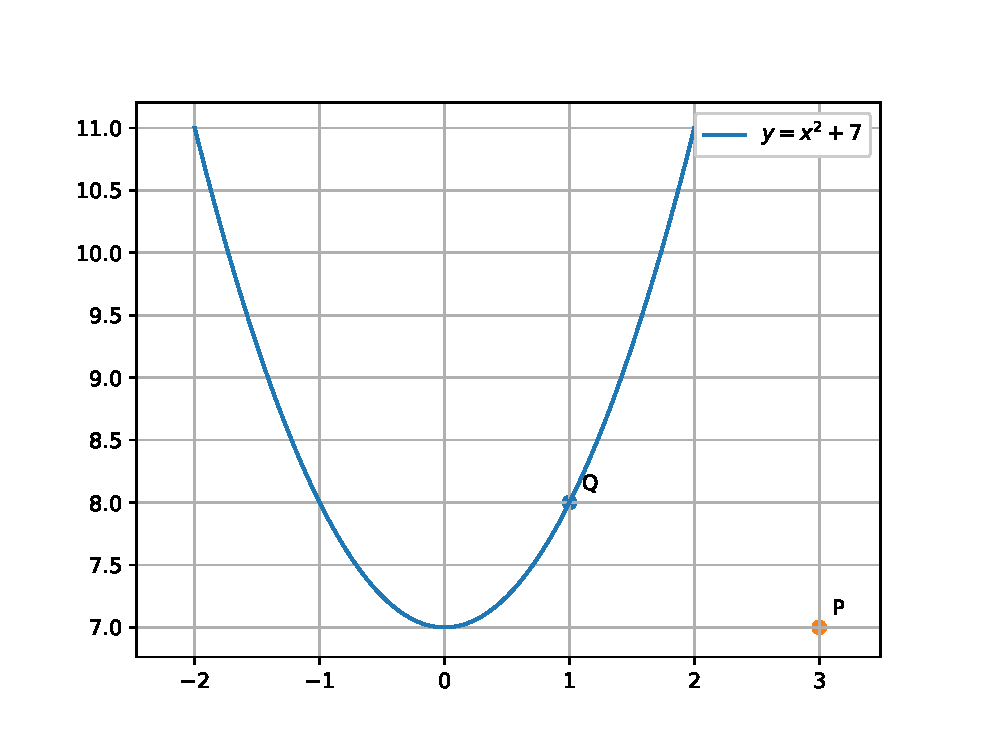
\includegraphics[width=\columnwidth]{./figs/qp_parab.eps}
\caption{ $\vec{Q}$ is closest to $\vec{P}$}.
\label{fig:qp_parab}
\end{figure}
%
%\item Frame 	
% as an optimization problem.
%\label{prob:qp_dist_pt_parab}
%\\
%
%\solution 
%From \eqref{eq2_1_line} and \eqref{eq2_1_circ}, 
%%
%\begin{align}
%r^2 & = (x_1-8)^2 + (3- x_1)^2 \\
%&= 2 x_1^2 - 22 x_1 + 73 \\
%\Rightarrow r^2 &= \frac{\brak{2x_1-11}^2 + 5^2}{2}
%\end{align}
%%
%which is minium when $x_1 = \frac{11}{2}, x_2 = \frac{7}{2}$.  The minimum value is $\frac{25}{2}$ and 
%the radius $r = \frac{5}{\sqrt{2}}$.
%	
%\begin{lstlisting}
%codes/optimization/lagmul.py
%\end{lstlisting}
\item Solve \eqref{eq:qp_dist_pt_parab_conv} using gradient descent.
%
\end{enumerate}
